\section{Introduction}
\label{sec:intro}
\IEEEPARstart{A}{utonomous} wheeled robots transport goods, inspect facilities, explore unfamiliar sites, and assist people indoors and outdoors. To navigate, a robot must estimate its pose from imperfect measurements, represent obstacles and traversable space, plan a route that its chassis can execute, and track that route as new observations arrive, while a team member must also reconcile its own observations with information received from teammates. Reliable operation therefore depends both on the individual algorithms and on the information that passes between estimation, mapping, planning, and control.

Degradation occurs when operating conditions depart from the assumptions of these algorithms. Cameras encounter poor texture or illumination, laser scans lack geometric variation, wheels slip, and moved furniture invalidates a stored map, whereas semantic predictions and delayed messages introduce errors into task interpretation and coordination. Ground-robot datasets document combinations of darkness, lift transitions, abrupt braking, and uneven terrain~\cite{P_M41,P_F11}. Beyond these sensing conditions, long-term deployments depend on charging, network availability, and operator assistance~\cite{P_M37}. Addressing these conditions requires methods that relate the quality of the available information to the actions that a robot can still execute safely.

Geometric, learned, and language-based methods address these requirements in combination. A semantic navigator may still rely on geometric localization and a local collision controller, just as a learned planner may retain a model-based feasibility test. Representative simultaneous localization and mapping (SLAM) systems~\cite{B_ORBSLAM32021,B_FASTLIO22022} and the dynamic-window~\cite{B_DWA1997} and timed-elastic-band~\cite{B_TEB2013} planners that recur as comparators~\cite{P_M06,P_M30} illustrate how these components assume different inputs and fail in different ways. Existing surveys examine individual aspects of the problem. They cover SLAM in extreme subterranean environments~\cite{B_SubTSLAM2024}, global LiDAR localization~\cite{B_GlobalLiDARLoc2024}, millimeter-wave radar in robotics~\cite{B_RadarSurvey2024}, automated-vehicle perception under adverse weather~\cite{B_AdverseWeather2023}, terrain traversability~\cite{B_Traversability2022}, safe learning in robotics~\cite{B_SafeLearning2022}, learned navigation policies~\cite{P_X04}, social navigation~\cite{B_SocialNav2023}, vision-and-language navigation~\cite{B_VLNSurvey2022}, collaborative SLAM~\cite{B_CSLAM2022}, and foundation models across embodiments~\cite{B_Foundation2024}. Each is organized around one function, task setting, or method family. Table~\ref{tab:related-reviews} lists their scopes alongside the cross-function connections developed here.

\begin{table*}[t]
\centering
\caption{Representative related surveys and the system-level connections examined in this review.}
\label{tab:related-reviews}
\surveytableformat
\begin{tabularx}{\linewidth}{@{}L{3.3cm}L{5.5cm}Y@{}}
\toprule
\textbf{Review} & \textbf{Main organizing subject} & \textbf{Connection developed in this survey} \\
\midrule
Ebadi et al. (2024)~\cite{B_SubTSLAM2024} & SLAM systems and lessons from the DARPA Subterranean Challenge & Degradation responses connected to recovery actions and task outcomes beyond estimator design \\
\addlinespace[3pt]
Yin et al. (2024)~\cite{B_GlobalLiDARLoc2024} & Global LiDAR localization, place retrieval, and cross-robot localization & Relocalization as a recovery action whose candidate must be validated before navigation resumes \\
\addlinespace[3pt]
Harlow et al. (2024)~\cite{B_RadarSurvey2024} & Millimeter-wave radar for motion estimation, localization, mapping, and object detection & Radar as an independent motion source when cameras or LiDAR degrade \\
\addlinespace[3pt]
Zhang et al. (2023)~\cite{B_AdverseWeather2023} & Weather effects on automated-vehicle sensors and the perception, fusion, and dataset responses & Sensing degradation traced through estimation to recovery and task outcomes \\
\addlinespace[3pt]
Sevastopoulos and Konstantopoulos (2022)~\cite{B_Traversability2022} & Estimation of whether terrain can be traversed & Pose uncertainty, vehicle limits, route choice, and motion outcomes \\
\addlinespace[3pt]
Brunke et al. (2022)~\cite{B_SafeLearning2022} & Learning-based control, safe reinforcement learning, and certification of learned policies & Safety filters judged by the state, input, and timing assumptions of their guarantees \\
\addlinespace[3pt]
Zhu and Zhang (2021)~\cite{P_X04} & Deep reinforcement learning for navigation & Relations between learned decisions, constraints, and deployment evidence \\
\addlinespace[3pt]
Mavrogiannis et al. (2023)~\cite{B_SocialNav2023} & Planning, behavior design, and evaluation for social robot navigation & Social constraints kept separate from collision geometry and tested under degraded perception \\
\addlinespace[3pt]
Gu et al. (2022)~\cite{B_VLNSurvey2022} & Tasks, methods, and future directions in vision-and-language navigation & Semantic decisions coupled to geometric execution, response timing, and fallback \\
\addlinespace[3pt]
Lajoie et al. (2022)~\cite{B_CSLAM2022} & Collaborative localization and mapping & Shared-state validity during disconnection, local operation, and reconnection \\
\addlinespace[3pt]
Firoozi et al. (2025)~\cite{B_Foundation2024} & Pretrained models across perception, decision-making, and control & Query timing, local constraints, and fallback in wheeled navigation \\
\bottomrule
\end{tabularx}
\end{table*}

\begin{figure*}[t]
\centering
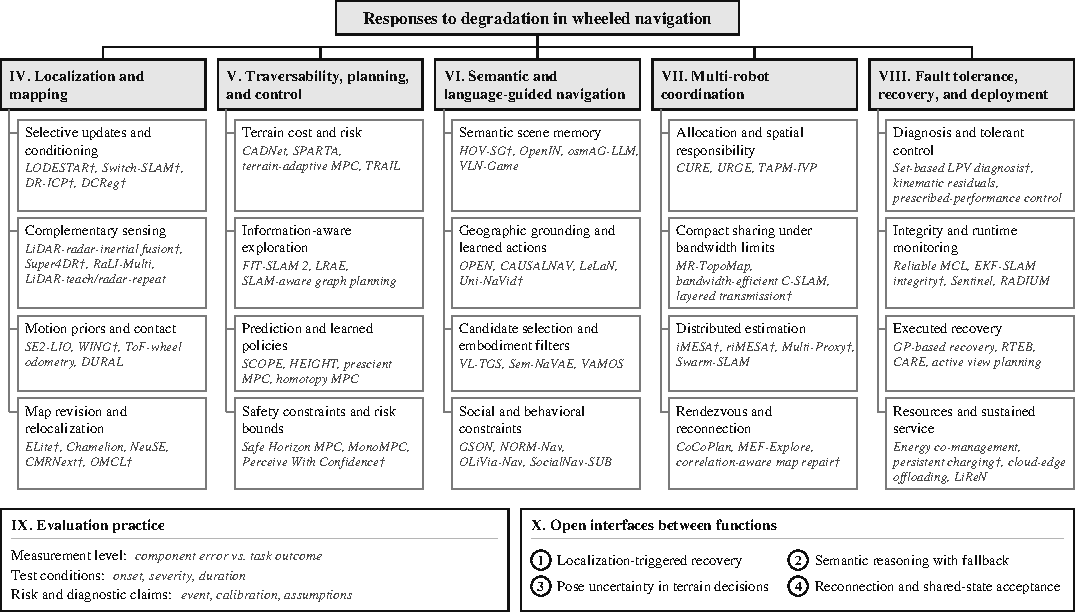
\includegraphics[width=\textwidth]{figures/fig-taxonomy.pdf}
\caption{Organization of the survey. Sections~IV--VIII group responses to degradation by navigation function, with representative methods listed under each response family. The methods are examples rather than complete lists, and $\dagger$ marks examples not evaluated on a wheeled robot or its data. Section~IX compares evaluation practice along three axes, and Section~X examines four interfaces between functions whose behavior under degradation remains insufficiently characterized.}
\label{fig:taxonomy}
\end{figure*}

This survey organizes the literature around three questions: which navigation assumption a degradation affects, how a method changes the information or action available to the robot, and what evidence connects that change to navigation performance. Fig.~\ref{fig:taxonomy} shows the resulting organization by navigation function, response family, and open interface. The main contributions of this survey are summarized as follows. First, this survey compares responses to degradation across five navigation functions together with their sensing, model, and action requirements, distinguishing component improvements from executed recovery. Second, it codes the evaluation evidence of the \CoreCount{} technical publications by navigation function and finds that, in this purposive sample, only \DegTaskShare\% report task outcomes under a named degradation condition. It also examines how platform, reference dependence, computation placement, and experimental design condition the interpretation of reported results. Third, it proposes four interfaces between existing methods that merit joint evaluation and outlines a matched comparison for each, namely localization-triggered recovery, semantic reasoning with fallback, pose uncertainty in terrain decisions, and shared-state acceptance after reconnection.

The remainder of this survey is organized as follows. Section~\ref{sec:background} introduces wheeled motion constraints, the navigation stack, and the sources of degradation, after which Section~\ref{sec:methodology} defines the scope and literature selection. Sections~\ref{sec:localization}--\ref{sec:reliability} develop the technical synthesis, Section~\ref{sec:evaluation} compares evaluation practice, Section~\ref{sec:challenges} presents open challenges, and Section~\ref{sec:conclusion} concludes this survey.
